\section{Results}
The results of the implementation are addressed in this section. They are reasonably representative for the average results. By reasonably, we mean that the simulation has been run enough times to see the that the results are only starting to converge, though the trend is fully visible. The results are divided into the two following sections: Simple Simulation and Advanced Simulation.

\subsection{Results with simple simulation}
The simple simulation is characterized by sensors being spread relatively even throughout the map. The rule is that a sensor cannot touch another sensor. When using the simple simulator each sensor can only sense its closest neighbours. 

Figure \ref{fig:simple-results1} illustrates the success of the fire interpreter. The light green color is where the actual fire is and where the interpreter predicted it to be. Thus it is the color of success. The dark green color is area where the interpreter thought it would be fire, but was not. The red parts are the actual fire which the interpreter did not predict.

\begin{figure}[here]
  \centering
      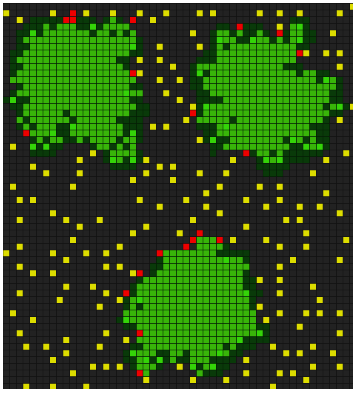
\includegraphics[width=0.7\textwidth]{discussion/graphics/results-simple-compare.png}
  \caption{The intense green is where the fire interpreter predicted fire correctly. The dark green is where the fire interpreter thought there were fire, but there were no fire present. Red dots are where there actually were fire, but the interpreter was unable to predict it.}
  \label{fig:simple-results1}
\end{figure}

\subsection{Results with advanced simulation}
The advanced simulation mimics the effect humidity and wind has on a fire. In addition, the sensors are spread more randomly than in the simple simulation. They can also sense with a larger range. The default range is two cells. The fire interpreter used the wind add-on in the kernel in the successful tests, while it was turned off in the tests which had less than ideal results. There are a number of parameters which has been tweaked to get good results. These different parameters makes it more difficult to get an accurate prediction. Figure \ref{fig:wind-advanced-bresenham-large} illustrates the predicted fire on top of the actual fire when the wind is blowing from west.

\begin{figure}[here]
  \centering
      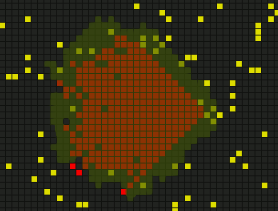
\includegraphics[width=0.5\textwidth]{discussion/graphics/wind-advanced-bresenham-large.png}
  \caption{The dark green overlay is where the fire interpreter predicted the fire to be. The red covered by the green overlay is where the fire interpreter predicted correctly and the red dots without any overlay is where there was fire, but did not predict.}
  \label{fig:wind-advanced-bresenham-large}
\end{figure}

The prediction is covering a larger area than the actual fire. This is because the sensors are sensing 2 cells away. In figure \ref{fig:wind-advanced-bresenham-large} this can be observed by viewing the right most predicted fire. The two sensors which are located beneath the right most predicted area are sensing fire and therefore the prediction is set from this point. The first cells north and south of this area has also been predicted to be on fire. This is because of Bresenham’s line algorithm which interprets these two cells to be on the outer boundary of the sensors sensing fire. The algorithms from computer graphics is used to make sure there are no holes inside the predicted fire and to prevent wind problem (chapter \ref{wind-problem}).

\begin{figure}[here]
  \centering
      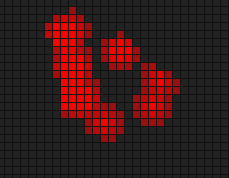
\includegraphics[width=0.5\textwidth]{discussion/graphics/advanced-without-wind-and-bresenham.png}
  \caption{Wind and graphical algorithms disabled in the advanced simulation creates holes and shows a lack wind direction.}
  \label{fig:advanced-without-wind-and-bresenham}
\end{figure}

Figure \ref{fig:advanced-without-wind-and-bresenham} illustrates what is happening when wind and the graphical algorithms are disabled. When we utilize the advanced simulation, the interpreter, with wind and graphical algorithms, has the best performace compared to the other tested solutions. The prediction with this setup reproduces the shape of the actual fire with a satisfactory result. The area of the shape is larger than the actual fire. The philosophy was always to air on the side of safety. Meaning that the fire interpreter aimed to detect all fires and as such a few false positives were deemed to be acceptable.